\documentclass[12pt, a4paper, bibliography=totoc]{scrreprt}


%\input{~/Latex/article/article_config.tex}
% personal data
\date{\today}


% language
\usepackage{polyglossia}
\setmainlanguage{english}
\setotherlanguages{german}
\usepackage{microtype}
\usepackage{dcolumn}

\usepackage[style=numeric,
			natbib=true,
			backend=biber]{biblatex}		%Bibliographie
\usepackage[autostyle=true,
			 german=quotes]
			 {csquotes}					%Anführungszeichen
\usepackage{blindtext}


%math and theorems
\usepackage{amsmath}
\usepackage{amssymb}
\usepackage{amsopn}					%Matheoperatoren
\usepackage[amsmath,thmmarks,hyperref]{ntheorem}
\usepackage{mathtools}
\usepackage{mathdots}					%Punkte
\usepackage{dsfont}
\usepackage{upgreek}					%Griechische Buchstaben
\usepackage{bbm}						%Mengensymbol
\usepackage{physics}					%Physiksymbole
\usepackage{relsize}						%Größenangaben
\usepackage[separate-uncertainty,
			per-mode=symbol]
			{siunitx}					%Einheiten
%\usepackage{tikz}						%Zeichnen
\usepackage{upgreek}					%Griechische Buchstaben
\usepackage{enumitem}
\setlist{nolistsep}


%useful packages
%\usepackage{geometry}
\usepackage{xcolor}
\usepackage{graphicx}
\usepackage{float}
\usepackage{csquotes}
\usepackage{todonotes}
\usepackage{booktabs}
\usepackage{array}
\usepackage[labelfont=bf]{caption}
\usepackage{wrapfig}
\usepackage{enumitem}
%\usepackage{xr} % cross referencing
%\usepackage{titling}
%\usepackage{titlesec}
%\usepackage[Bjornstrup]
%			{fncychap}					%Kapitellayout


\setmainfont{Linux Libertine O}
\setsansfont{Linux Biolinum O}

\usepackage{scrhack}					%Verbesserung Pakete
\usepackage{xltxtra}						%fontec


\newcommand{\im}{\mathrm{i}}
\newcommand{\e}{\mathrm{e}}
\renewcommand{\pi}{\uppi}
\renewcommand{\epsilon}{\varepsilon}


\addbibresource{bibliography.bib}

%color settings
\definecolor{myred}{RGB}{196,19,47} 
\definecolor{myblue}{RGB}{0,139,139}


%appendix
\usepackage[toc,page]{appendix}

%killing indent
\setlength{\parindent}{0pt}
\usepackage{multicol}
\usepackage{siunitx}
\usepackage{hyperref}


\title{Studying the $Z$ Boson with the ATLAS Detector at the LHC}
\author{Aaron Mielke \& Thomas Ackermann}

\begin{document}


\begin{center}
	\makeatletter
	\thispagestyle{empty}
	
	\begin{figure}[H]
	\flushright
	
\includegraphics[width=0.35\textwidth]{fig/logo}
	\end{figure}
	
	\vspace{-30mm}
	
	\begin{flushleft}
	\large{\textbf{Fortgeschrittenen Praktikum} \\
		Summer term 2019} \\
	\end{flushleft}
	
	\vspace{5mm}
	
	\rule{\textwidth}{0.2pt}

	\vspace{50mm}
	\Huge\textbf{\@title} \\
	\vspace{10mm}
	\large{\@author} \\
	\normalfont
	
	\vspace{2mm}
	
	\makeatother
\end{center}

\normalsize
\newpage

\tableofcontents


\chapter*{Abstract}
This is the abstract





\chapter{Introduction}

The main goal of the lab course is to analyze data from the ATLAS experiment and 
to calculate the invariant mass of the $Z$ Boson. 

\section{The Standard Model of Particle Physics}

The Standard Model of Particle Physics is the summarization of the known structure of matter.
It implies, that matter is composed of the twelve elementary fermions with spin $\frac{1}{2}$, which are the quarks and leptons. Each of these particles has a corresponding anti-particle, which are equal except their opposite charge.
\\
\\
Maybe the table?
\\
\\
The interaction between these particles is divided in three categories and are mediated by bosons carrying spin 1. The weak force exchange particles are the massiv $Z$ and $W^{\pm}$ bosons, the massless photons for the electromagnetic force and eight massless gluons are mediating the strong force. 
 
\section{Drell-Yan Process}
A $Z$ Boson can be created during the so called ``Drell-Yan'' Process. This process happens predominatly in proton-proton collisions.
When a quark and an anti-quark collide either a virtual photon or a $Z$ Boson can be produced. 
The $\gamma*$ or the $Z$ can then split into a lepton and its anti-particle partner like electron-positron or muon and anti-muon.
The sum of the lepton and anti-particle partner momenta will then add up to the former boson momentum. A peak around 90 GeV will be observed correspondig to the $Z$ boson. 

\section{ATLAS Detector}
The Detector consists of three main components: inner detector, calorimeters and the muon spectrometer. They are onion-like constructed. 
The inner detector, the innermost layer, is mainly used to reconstruct the trajectories of electrically charged particles and to determine their momentum. With three aswell onion-like ordered tracking detectors, the pixel detector, the semi-conductor tracker and the transition radiation tracker, the inner detector can measure charged particles in a range of $|\eta| < 2.5$ and a $p_{T} > 400$ MeV.\\

The electromagnetic and the hadronic calorimeter allow to reconstruct the shower shapes of the showers from electromagnetically and strongly interacting particles. They are designed to contain the whole shower and cover a range up to $|\eta| < 4.9$. A precise energy measurement is possible.\\

The outermost layer is the muon spectrometer. Muons would espace the ATLAS detector without it and can now be tracked. 


\chapter{Experimental procedure}

\section{Get to known the data}
Before starting with the computation of the mass of the $Z$ bosons. One has to make oneself familiar with the provided data from the ATLAS detector. The given data is preselected. One only has data from events where a primary vertex was found and at least one lepton has to have a minimal transvers momnetum of $p_{T} = 25$ GeV.

\subsection{Particle entrance}
\begin{figure}
	\centering
	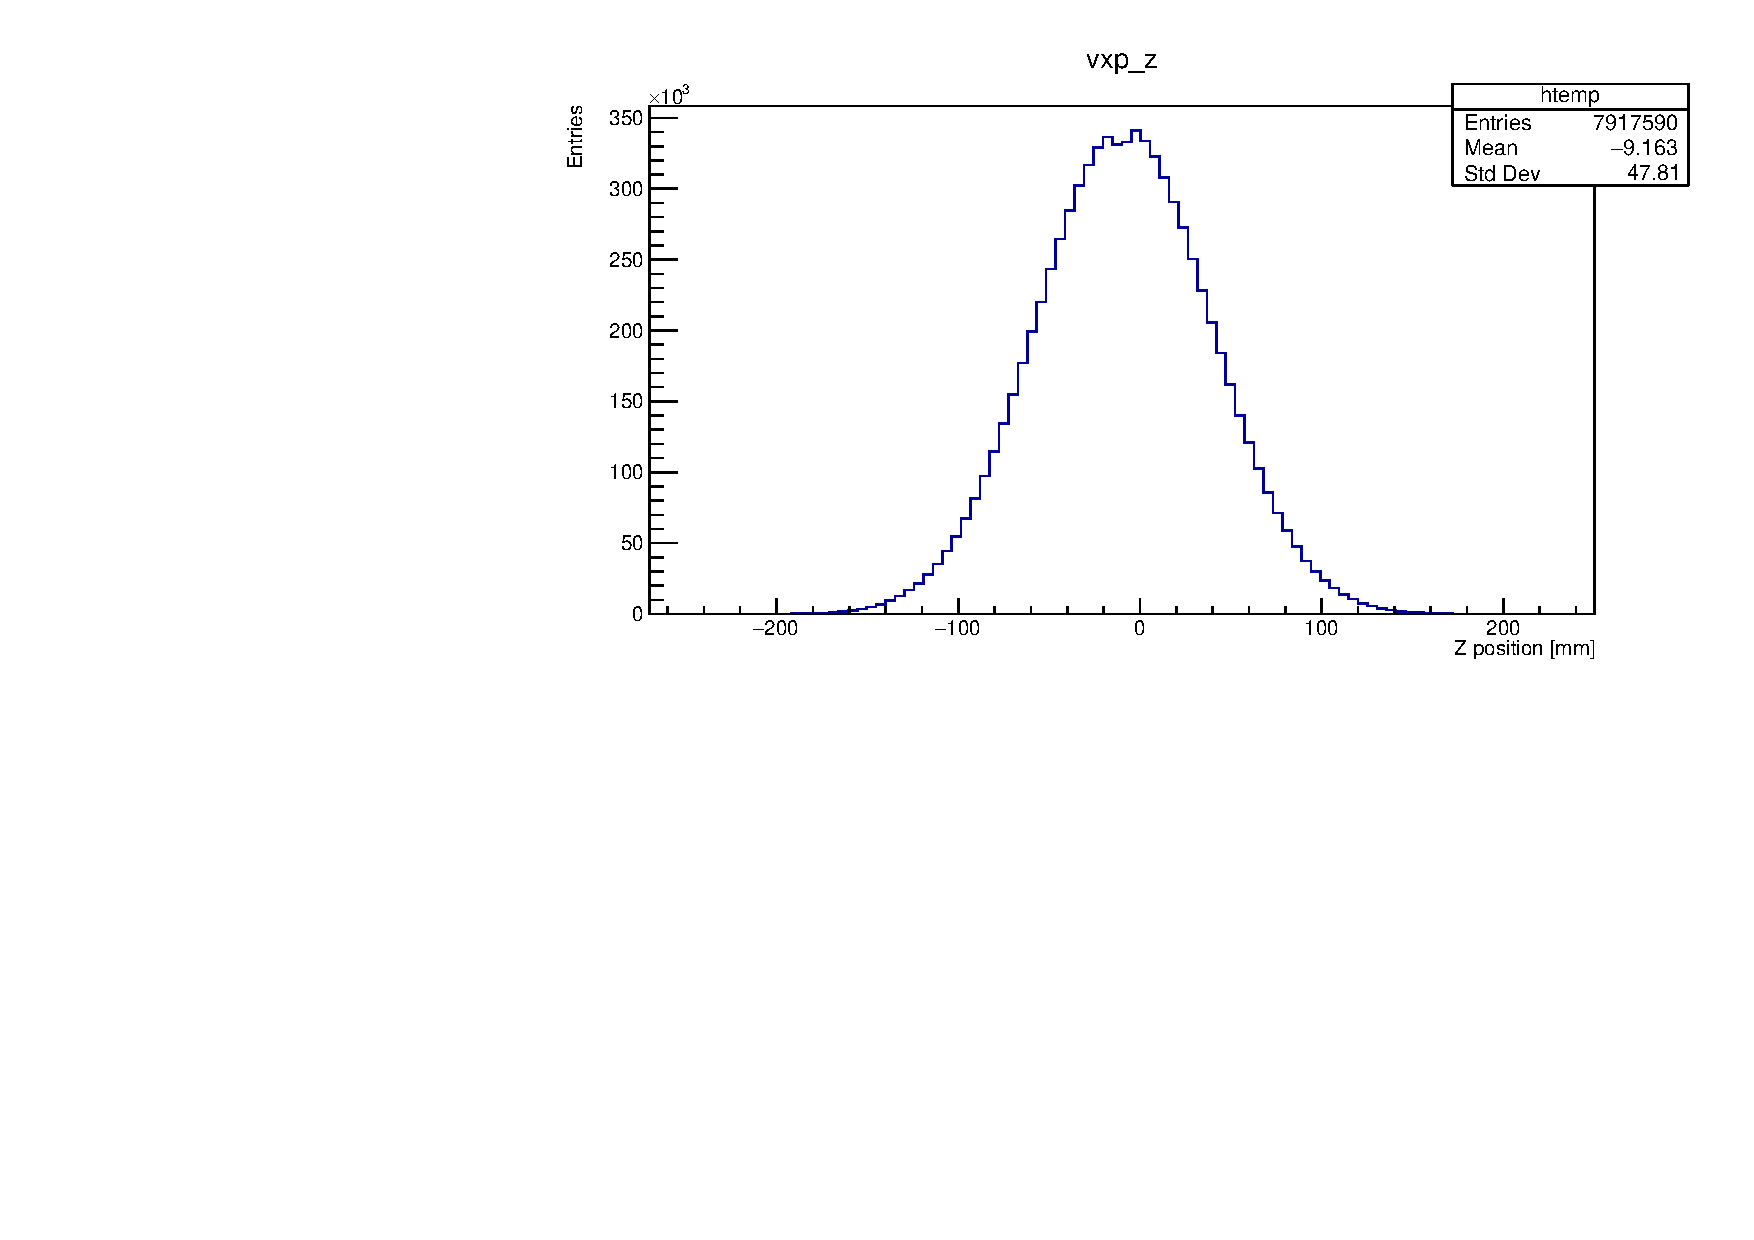
\includegraphics[scale=0.5]{fig/vxp_z_redo.pdf}
	\caption{z-postion distribution, particle entrence in ATLAS detector}
	\label{vxp_z}
\end{figure}
To check where the particle enter the detector, one can evaluate the given date for the vxp\_z variable. The results are shown in~\ref{vxp_z}. The mean is shifted for $-9$ mm. This confirms, that the given data is from 2012. The collision of bunchs was not calibrated to the $0.0$ position back then.
Left and right to the mean are two maxima, which corresponds with the assumption above. A momentum change of 90 degrees is impossible and most of the collisions take place at the place of the first intersection.

\subsection{leptons per event}
\begin{figure}
	\centering
	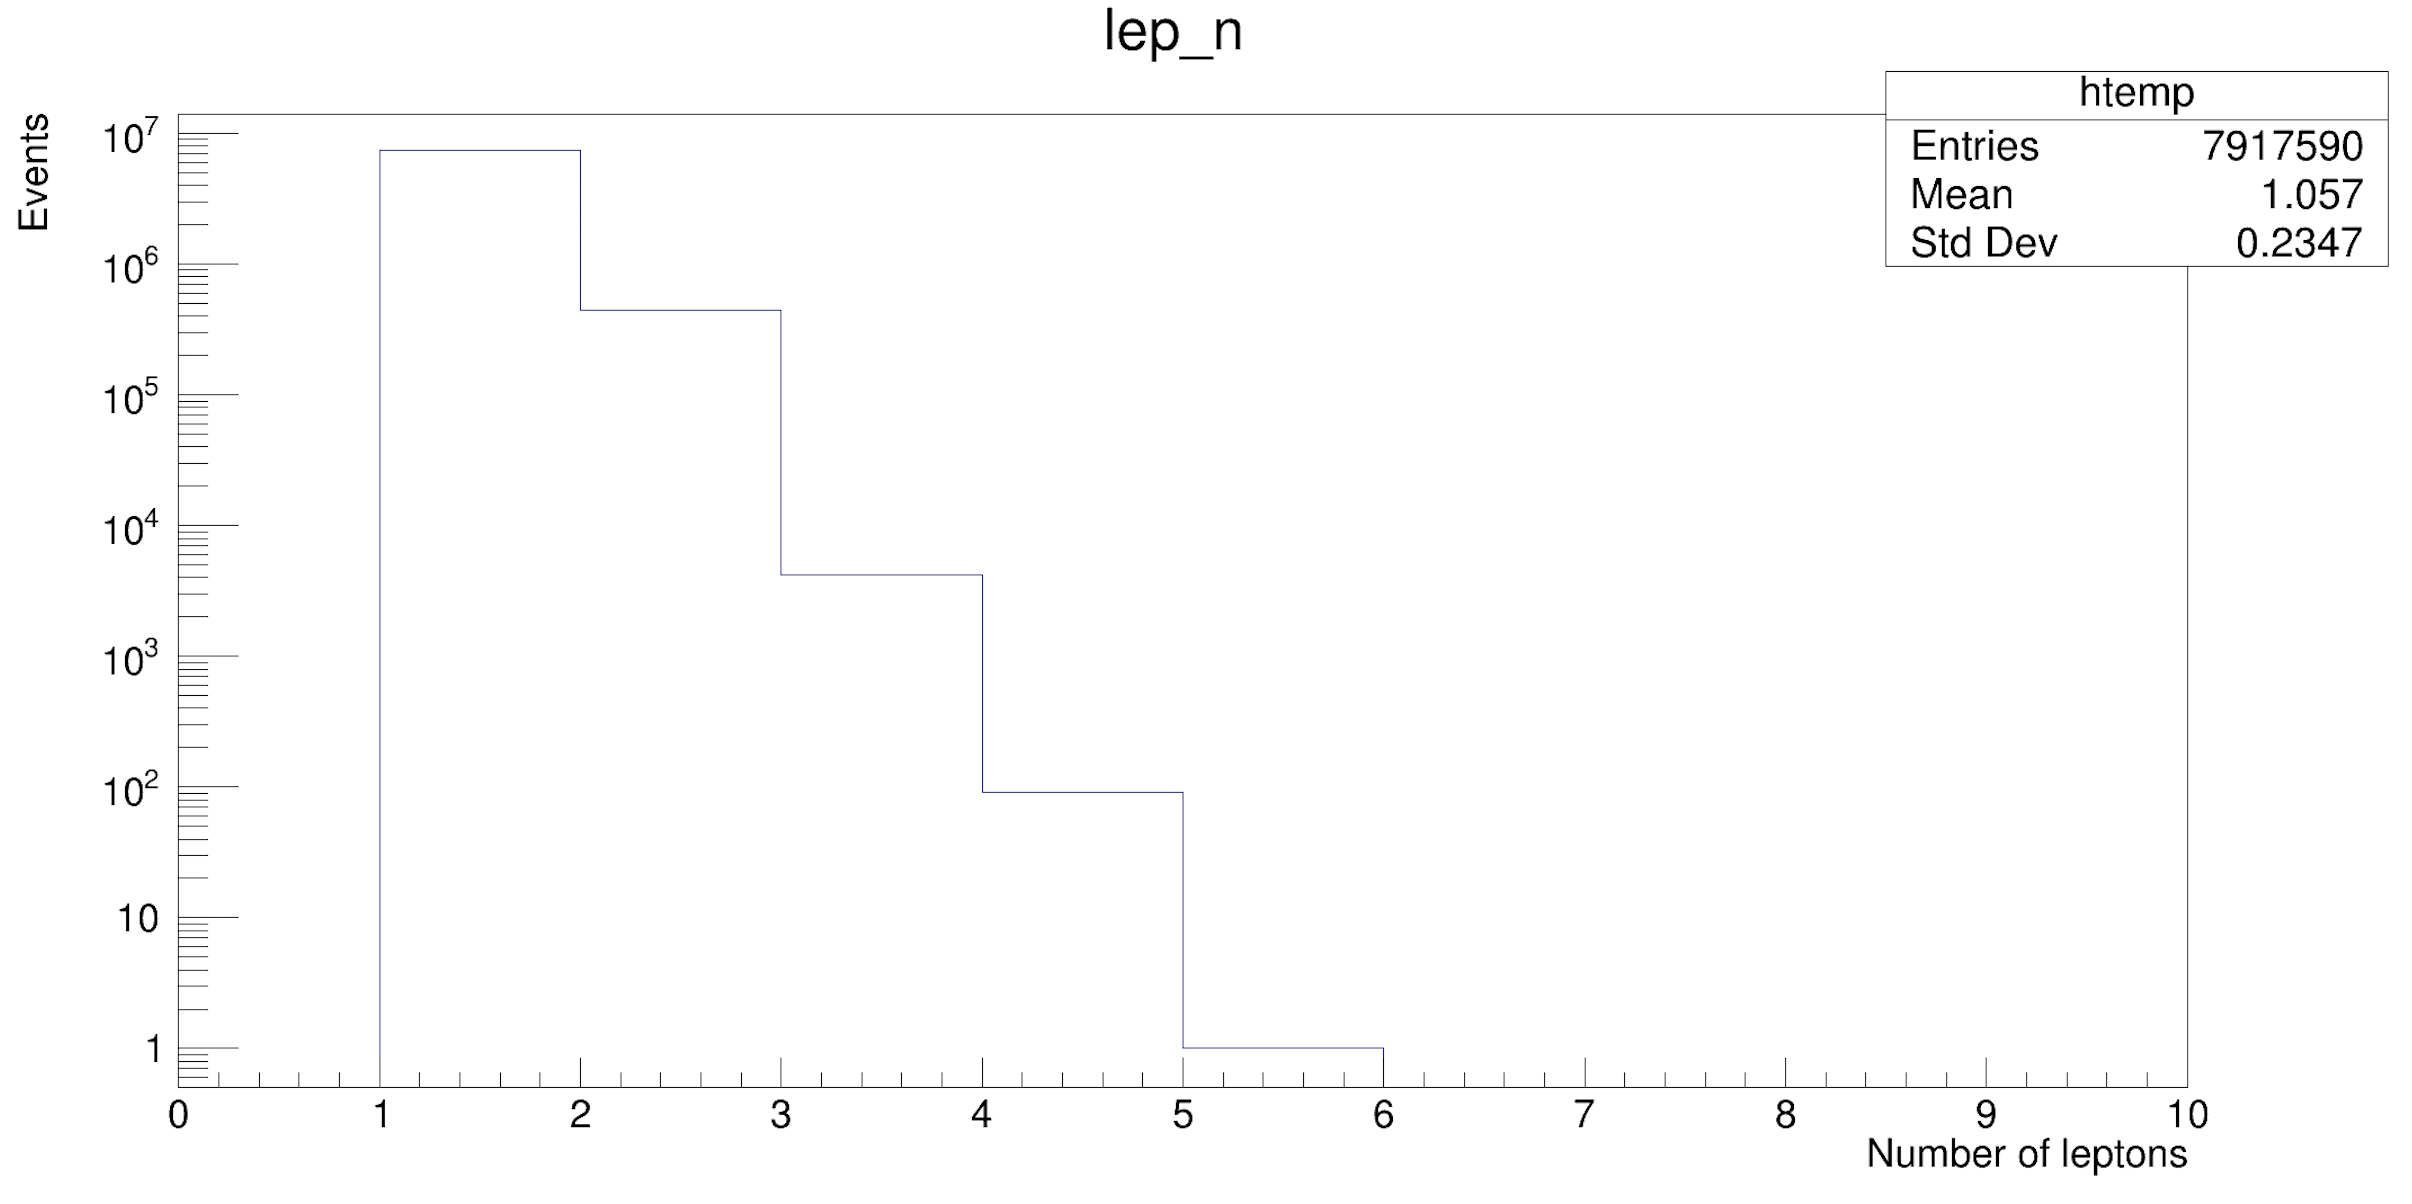
\includegraphics[scale=0.15]{fig/number_produced_leptons.png}
	\caption{leptons recorded per event}
	\label{lep_n}
\end{figure}
To figure out, if one found an $Z$ decay, one analysis the leptons per event value of the data[\ref{lep_n}].
Around the wanted 2 leptons, one gets many events with 1 and 3 leptons. For this events to happen, one needs a $W^{\pm}$ decay involved.

Feynmann diagramms ?

\subsection{data of the leptons}
the stored data about transvers impuls, the $\phi§$ degree and $\eta$ varible provide information about all the leptons recorded by the ATLAS detector and accordinlgy has more entries than the former analyzed data variables.

\section{Calculation of the invariant mass of the $Z$ boson}

\subsection{title} 
\nocite{*}
\appendix
\printbibliography

\end{document}

